\documentclass{paris17}
\usepackage{amsmath}
\usepackage{graphicx}
\usepackage{graphicx}
\usepackage{caption}
\usepackage{subcaption}
\usepackage{floatrow}
% Table float box with bottom caption, box width adjusted to content
\newfloatcommand{capbtabbox}{table}[][\FBwidth]
\usepackage{capt-of}% or \usepackage{caption}
\usepackage{booktabs}
\usepackage{varwidth}


\begin{document}

\section{Introduction}

Propagating wavefields using explicit finite difference method is the kernel of reverse time migration (RTM) and high-end velocity algorithms in seismic applications. In recent decades there has been a significant increase of interest in the seismic exploration community to reconstruct the image of the underground in larger regions and higher resolutions, especially in the elastic media. As a result the optimizing methods to improving the performance of the wavefield propagation are in great demands.



%As the Earth attenuates the seismic signals in real Earth materials, an accuracy wavefield modeling approach needs to account for the effects of attenuation and velocity dispersion \cite[]{zhu2014theory}.

One approach to improve the performance of modeling is to recognize that the earth attenuates seismic energies, in which case, we can ignore higher and higher frequencies and still obtain an accurate image\cite[]{Clapp.sep.111.bob3} when we push the wavefield down in depth. By using coarser sampling at large time steps,  the performance for downward continuation based approaches which are done frequency by frequency can be significantly improved.

The concept of the constant Q model introduced by \cite{Kjartansson.sep.23} are used to approximate the attenuation. However, the formulation for computing the time derivative for the constant Q model proposed by Podlubny requires to store wavefields from previous values to present time \cite[]{podlubny1998fractional}, which is impractical for real seismic modeling in terms on memory capacities on modern computers. Zhu developed a constant-Q wave equation using fractional Laplacian operators to avoid the need of storing the past values of the wavefields \cite[]{zhu2014theory}. However, the proposed method is for 2D viscoelastic case and the computation of fractional Laplacian is expensive compared with the conventional FD methods.

Meanwhile, the Nvidia Graphic Processing Units (GPUS)  have achieved great successes in many domains. In seismic application, GPUs are employed as high-performance computing accelerators for key seismic modeling, imaging and inversion kernels due to their high memory bandwidth and a large number of processing units \cite[]{ohmer2005implementation,he2015gpu}.

This work proposes a high performance design of accelerating the wavefield propagation in 3D elastic media by approximating the constant Q propagation on multiple Nvidia GPUs. We first propose the Q approximation formulation by extending the formulation from the 2D viscoelastic to the 3D viscoelastic case where the fractional Laplacian is approximated to the conventional Laplacian and the dispersion term is ignored.  Optimization strategies from different aspects (memory, occupancy, and overlapping) are performed to form a high performance modeling kernel on multiple GPUs. To further improve the performance, a couple of tricks are also applied to reduce the total computation. Combining all the optimization schemes, we can achieve a significant speedup of the 3D elastic wave propagation by 60 to 200 times over a highly optimized 24-core CPU solution.

\section{Method and Theory}

%\subsection{Modeling}

%Explicit finite difference modeling is constrained by figuring  out a sampling in time and space that results in stable propagation and does not create dispersive events.  For stability the Courant-Friedrichs-Lewy condition \cite[]{courant1967partial} must be met.  For stability, we have $v_{max}\frac{dt}{d_{min}} < .5$, where  $v_{max}$ is the maximum velocity; $dt$ is the

%Stability is a function of limiting what percentage of a grid cell energy can move in one time step. Stability is therefore a function of the maximum velocity $v_{max}$, the minimum spatial sampling $d_{min}$, and the time step $dt$.


%The stability condition pushes one to use larger spatial sampling (faster, but less resolution) and/or finer time sampling (more expensive).  Dispersion, on the other hand, is a function of the minimum velocity $v_{min}$, the maximum frequency $f_{max}$, and the maximum spaital sampling $d_{max}$.   To avoid grid dispersion we need to  sample a given frequency with a minimum number of points.  There isn't a consensus on the minimum number
%of points. For the purpose of this paper I will require  3.2  points therefore, we have $\frac{v_{min} }{f_{max}d_{max}} > 3.2 \label{eq:dispersion}$.

%The dispersion constraint pushes us towards smaller (more expensive) spatial sampling, because of the stability constraint, and results in smaller the steps.  Minimizing dispersion is the real reason for the expense of finite differences.  To avoid grid dispersion and achieve the same level of stability the number of operations increase by the fourth power (three due to space sampling and one for time).

%Attenuation varies as a function of frequency and earth materials. The first approximation I am going to use is the concept of the constant Q model introduced by \cite{Kjartansson.sep.23}.  Q is defined as $Q=2 \pi \left( \frac{E}{\partial E}\right)$, where $\frac{E}{\partial E}$ is the fraction of energy lost per cycle. The larger the $Q$ value, the less energy loss per cycles.  The constant Q assumption assumes that energy dies out is a function of the number of wavelengths traveled through a medium. The higher the frequency, the faster the energy is attenuated.

\subsection{Constant Q formulation}

Our theory is built on the foundation of \cite[]{zhu2014theory}. It is a time-domain differential equation for modeling seismic wave propagation in constant-Q viscoelastic media based on fractional spatial derivatives, specifically Laplacian differential operators of fractional order.  The stress–strain relation is derived from the classical equation expressed in terms of fractional time derivatives. The formulation has the advantage of not requiring additional field variables that increase the computer time and storage significantly \cite[]{zhu2014theory}.

We first extend the formulation of \cite[]{zhu2014theory} from the 2D viscoelastic case to the 3D viscoelastic case. Note that the Laplacian differential operators of fractional order bring extra computational costs to the elastic modeling, we approximate it with the conventional Laplacian operators, which significantly reduces the computing complexities. Also, we further reduce the computational costs by ignoring the dispersion terms because it make little effects compared to the attenuation of the signals. As a result, our equations are then

\begin{equation}
\begin{bmatrix} \sigma_{11}\\ \sigma_{22}\\ \sigma_{33} \end{bmatrix} = \begin{bmatrix} \frac{\partial \tau_p^{(1)}}{\partial t} + c_{11} & \frac{\partial \tau_p^{(1)}}{\partial t} - 2\frac{\partial \tau_s^{(1)}}{\partial t} +c_{12}& \frac{\partial \tau_p^{(1)}}{\partial t} - 2\frac{\partial \tau_s^{(1)}}{\partial t} +c_{13} \\ \frac{\partial \tau_p^{(2)}}{\partial t} - 2\frac{\partial \tau_s^{(2)}}{\partial t} +c_{12}& \frac{\partial \tau_p^{(2)}}{\partial t} + c_{22} & \frac{\partial \tau_p^{(2)}}{\partial t} - 2\frac{\partial \tau_s^{(2)}}{\partial t} +c_{23}\\ \frac{\partial \tau_p^{(3)}}{\partial t} - 2\frac{\partial \tau_s^{(3)}}{\partial t} +c_{13} & \frac{\partial \tau_p^{(3)}}{\partial t} - 2\frac{\partial \tau_s^{(3)}}{\partial t} +c_{23} & \frac{\partial \tau_p^{(3)}}{\partial t} + c_{33} \end{bmatrix} \begin{bmatrix} \epsilon_{11}\\ \epsilon_{22}\\ \epsilon_{33} \end{bmatrix}
\end{equation}

\begin{equation}
  \sigma_{12} = \left ( 2\frac{\partial}{\partial t} \left( \frac{c_{11}-c_{12}}{2}c_s^{(2\gamma_s-1)}\sin(\pi\gamma_s) \right) + c_{66} \right )\times \epsilon_{12}
\end{equation}

\begin{equation}
  \sigma_{13} = \left ( 2\frac{\partial}{\partial t} \left( \frac{c_{33}-c_{13}}{2}c_s^{(2\gamma_s-1)}\sin(\pi\gamma_s) \right) + c_{55} \right )\times \epsilon_{13}
\end{equation}

\begin{equation}
  \sigma_{23} = \left ( 2\frac{\partial}{\partial t} \left( \frac{c_{22}-c_{23}}{2}c_s^{(2\gamma_s-1)}\sin(\pi\gamma_s) \right) + c_{44} \right )\times \epsilon_{23}
\end{equation}

\begin{equation}
  \tau_p^{(1)} = c_{11}C_p^{2\gamma_p - 1}\sin(\pi \gamma_p)
\end{equation}

\begin{equation}
  \tau_s^{(1)} = \frac{c_{11} - c_{13}}{2}C_s^{2\gamma_s - 1}\sin(\pi \gamma_s)
\end{equation}

\begin{equation}
  \gamma_{p,s}=\frac{1}{\pi}\tan^{-1}(\frac{1}{Q_{p,s}})
\end{equation}

where $\sigma$ is the stress tensor; $\epsilon$ is the strain tensor; $c_{ij}$ is the forth-order stiffness tensor; $C_p$ and $C_s$ are the velocities of P-wave and S-wave. $Q_{p,s}$ is the constant factor for the attenuation of P-wave and S-wave respectively. Note that we only present how $\tau_p^{(1)}$ and $\tau_s^{(1)}$ are derived, $\tau_p^{(2)}$,$\tau_p^{(3)}$, $\tau_s^{(2)}$ and $\tau_s^{(3)}$ can be derived in a similar way.

The reason why our constant Q formulation is relatively computationally economic are: (1) The fractional Laplacian is approximated to the conventional Laplacian. (2) The dispersion term is ignored. (3) We preserve the original workflow of elastic modeling while only adding a few terms in the calculation of stress tensors from train tensors.

\subsection{GPU Optimizations}

The reason why GPUs outperforms CPUs significantly on many scenarios is that the architecture of GPUs favors throughput of many data-parallel tasks over the latency of a single thread. We have an efficient parallel design on the GPU platform with three main strategies.

Firstly, we fully utilize the different hierarchical memory of the GPU. We keep a set of constant variables such as the derivative coefficients in the constant memory and the read-only cache. As the 64KB first-level cache can be configured as different combinations between L1 cache and shared memory, we configure it dynamically based on different computing scenarios. For the stencil computation, we configure the first-level cache by setting the sizes of shared memory and L1 cache to be 48 KB and 16 KB, respectively, which achieves a high computation performance based on P. Micikevicius’ 3D stencil design. For others, we prefer to configure the first-level cache as L1 cache if we don't use shared memory explicitly.

Secondly, we carefully tune the number of registers per thread to maximize the occupancy of GPUs. Since the access pattern of GPU global memory in the stencil kernel is irregular, the more threads are busy, the less latencies it is for memory access. However, as the number of registers is limited in a streaming multiprocessor (SM), increasing the number of registers per threads will decrease the number of active warps. So it is important to have a strategy to balance them. We first remove the intermediate variables to reduce the number of registers per threads. Then we dynamically tracking the performance by adjusting the block size and the \emph{maxrregcount} compiler option.

Thirdly, we design a computation and communication overlapping scheme to maximize the concurrency of different resources. The entire wavefield domain is divided into 4 subdomain, each assigning to a GPU shown in Figure \ref{fig:domain-decomposition}. Note that we need ghost cells to store and exchanges the halos, denoted by the arrows. In each subdomain, we further divide it into three parts, the halo part, the outer part and the inner part shown in Figure \ref{fig:task-decomposition}. The computation of inner and outer parts are assigned to different CUDA streams so that they are executed concurrently. When the computation of the outer part is finished, the GPU starts exchanging halos with its neighbors. In this way, the computation of the inner part can hide the communication shown in Figure \ref{fig:overlap}.

\begin{figure}[h]
    \centering
    \begin{subfigure}[b]{0.3\textwidth}
        \centering
        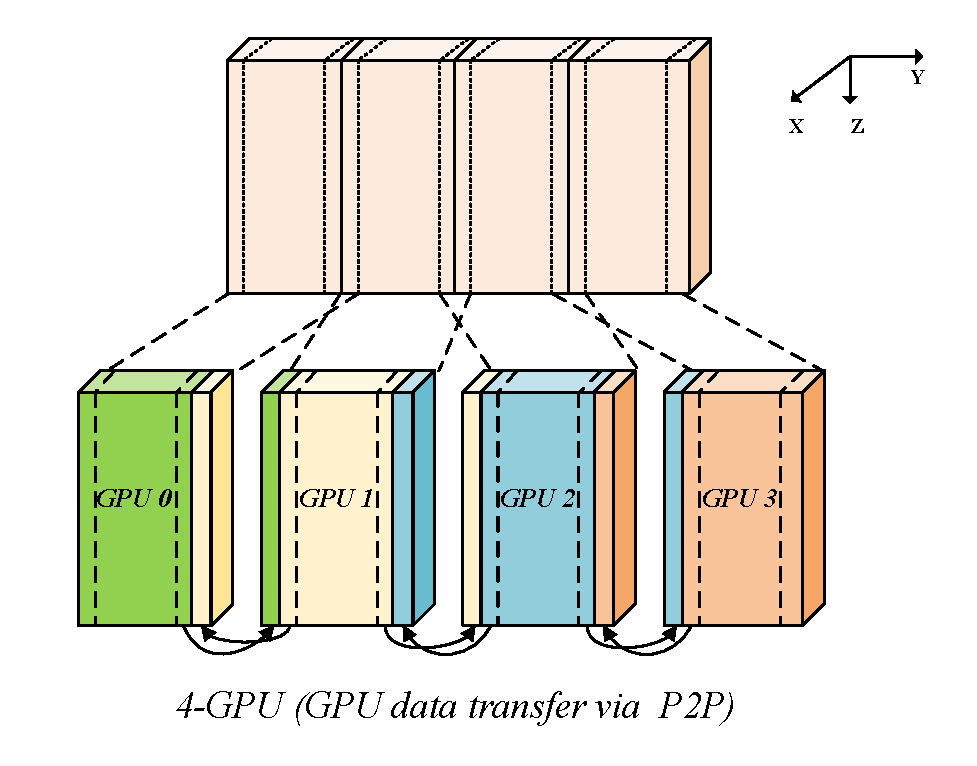
\includegraphics[height=1.3in]{./fig/domain-decompose.pdf}
        \caption{Domain decomposition}
        \label{fig:domain-decomposition}
    \end{subfigure}%
    ~
    \begin{subfigure}[b]{0.3\textwidth}
        \centering
        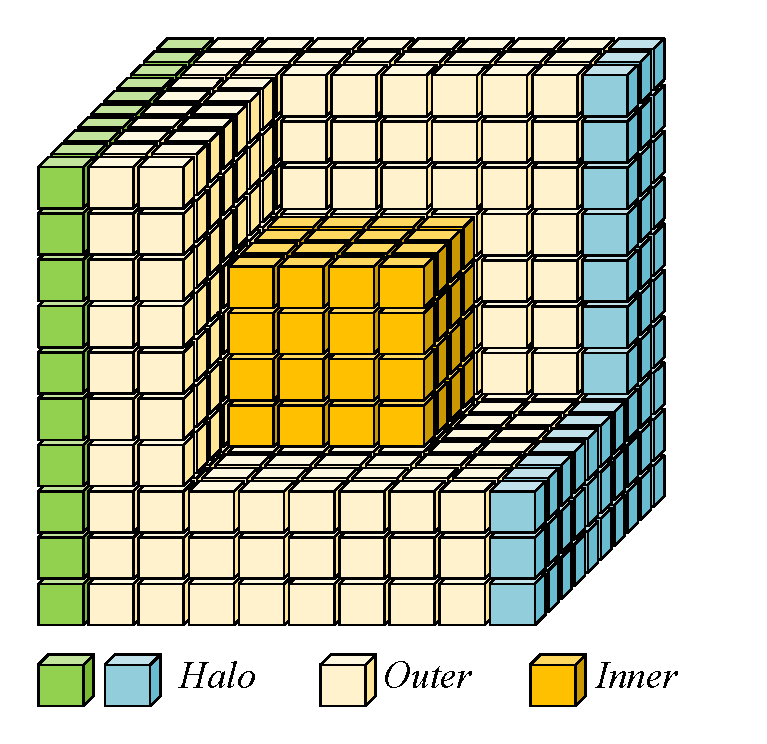
\includegraphics[height=1.3in]{./fig/inner-outer.pdf}
        \caption{Task decomposition}
        \label{fig:task-decomposition}
    \end{subfigure}
    ~
    \begin{subfigure}[b]{0.3\textwidth}
        \centering
        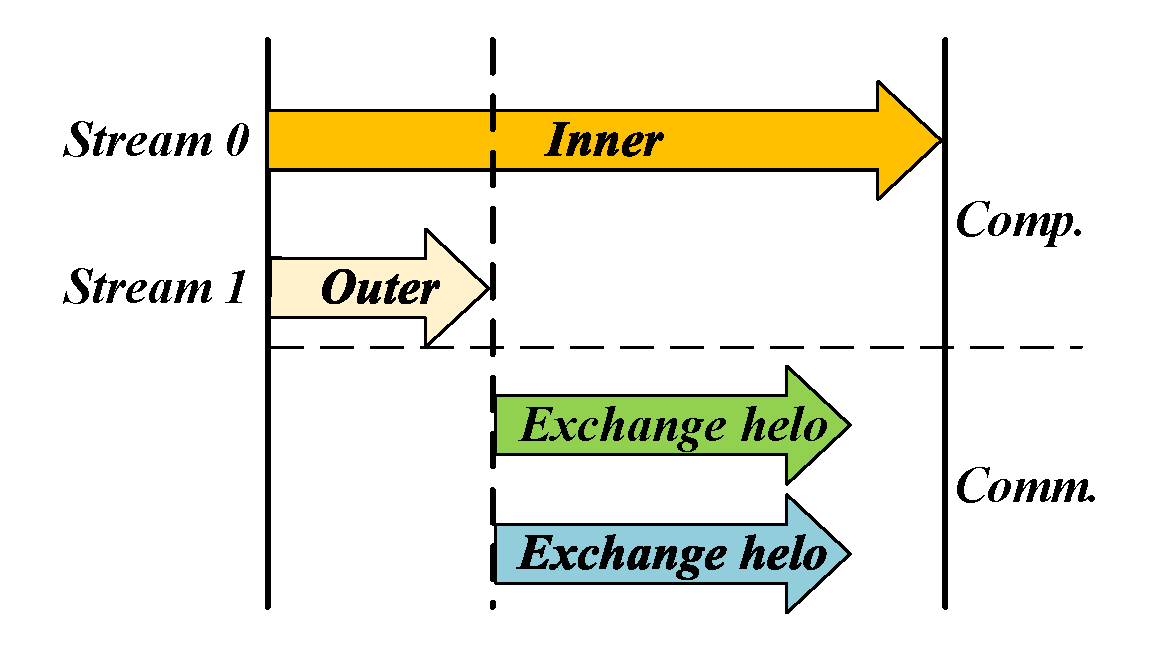
\includegraphics[height=1.1in]{./fig/overlap.pdf}
        \caption{Comp. \& Comm. overlapping}
        \label{fig:overlap}
    \end{subfigure}
    \caption{Computation and communication overlapping over multiple GPUs.}
\end{figure}

\subsection{Other Optimization Tricks}

Apart from the GPU-based optimization, we also apply another two approaches to further improve the performance.  After we taking the energy attenuation into consideration, we can ignore the frequencies that have attenuated. As a result, the grid cells and the time steps get larger as the wavefield propagate in time. We can achieve significant speedup when we resample the velocities and wavefields to coarser grids, especially recording the longer time step. Using the above approach, the early time steps dominate the computation. We eliminate the bottleneck by applying another trick that we recognize that it is not necessary to propagate the wavefields significantly away from the source at early times. We eliminate the update of the wavefields where the waves have not reached so far.



\section{Experiments}

\subsection{Q Effects}
Experiments for demonstrating the functionality of applying the Q effects as well as  the performance with different optimization tricks are carried out in this paper. Figure \ref{fig:with-attenuation} shows a slice of the z-component of the 3D wavefield using standard elastic wave equation at time 0.9 seconds while the Figure \ref{fig:without-attenuation} shows the wavefields with the constant Q effect ($Q_s=Q_p=20$) added. The wave front in Figure \ref{fig:with-attenuation} is weaker. The spectrum of the wavefields gives a better illustration, which is shown in Figure \ref{fig:spectrum}.

\begin{figure}[h]
    \centering
    \begin{subfigure}[b]{0.3\textwidth}
        \centering
        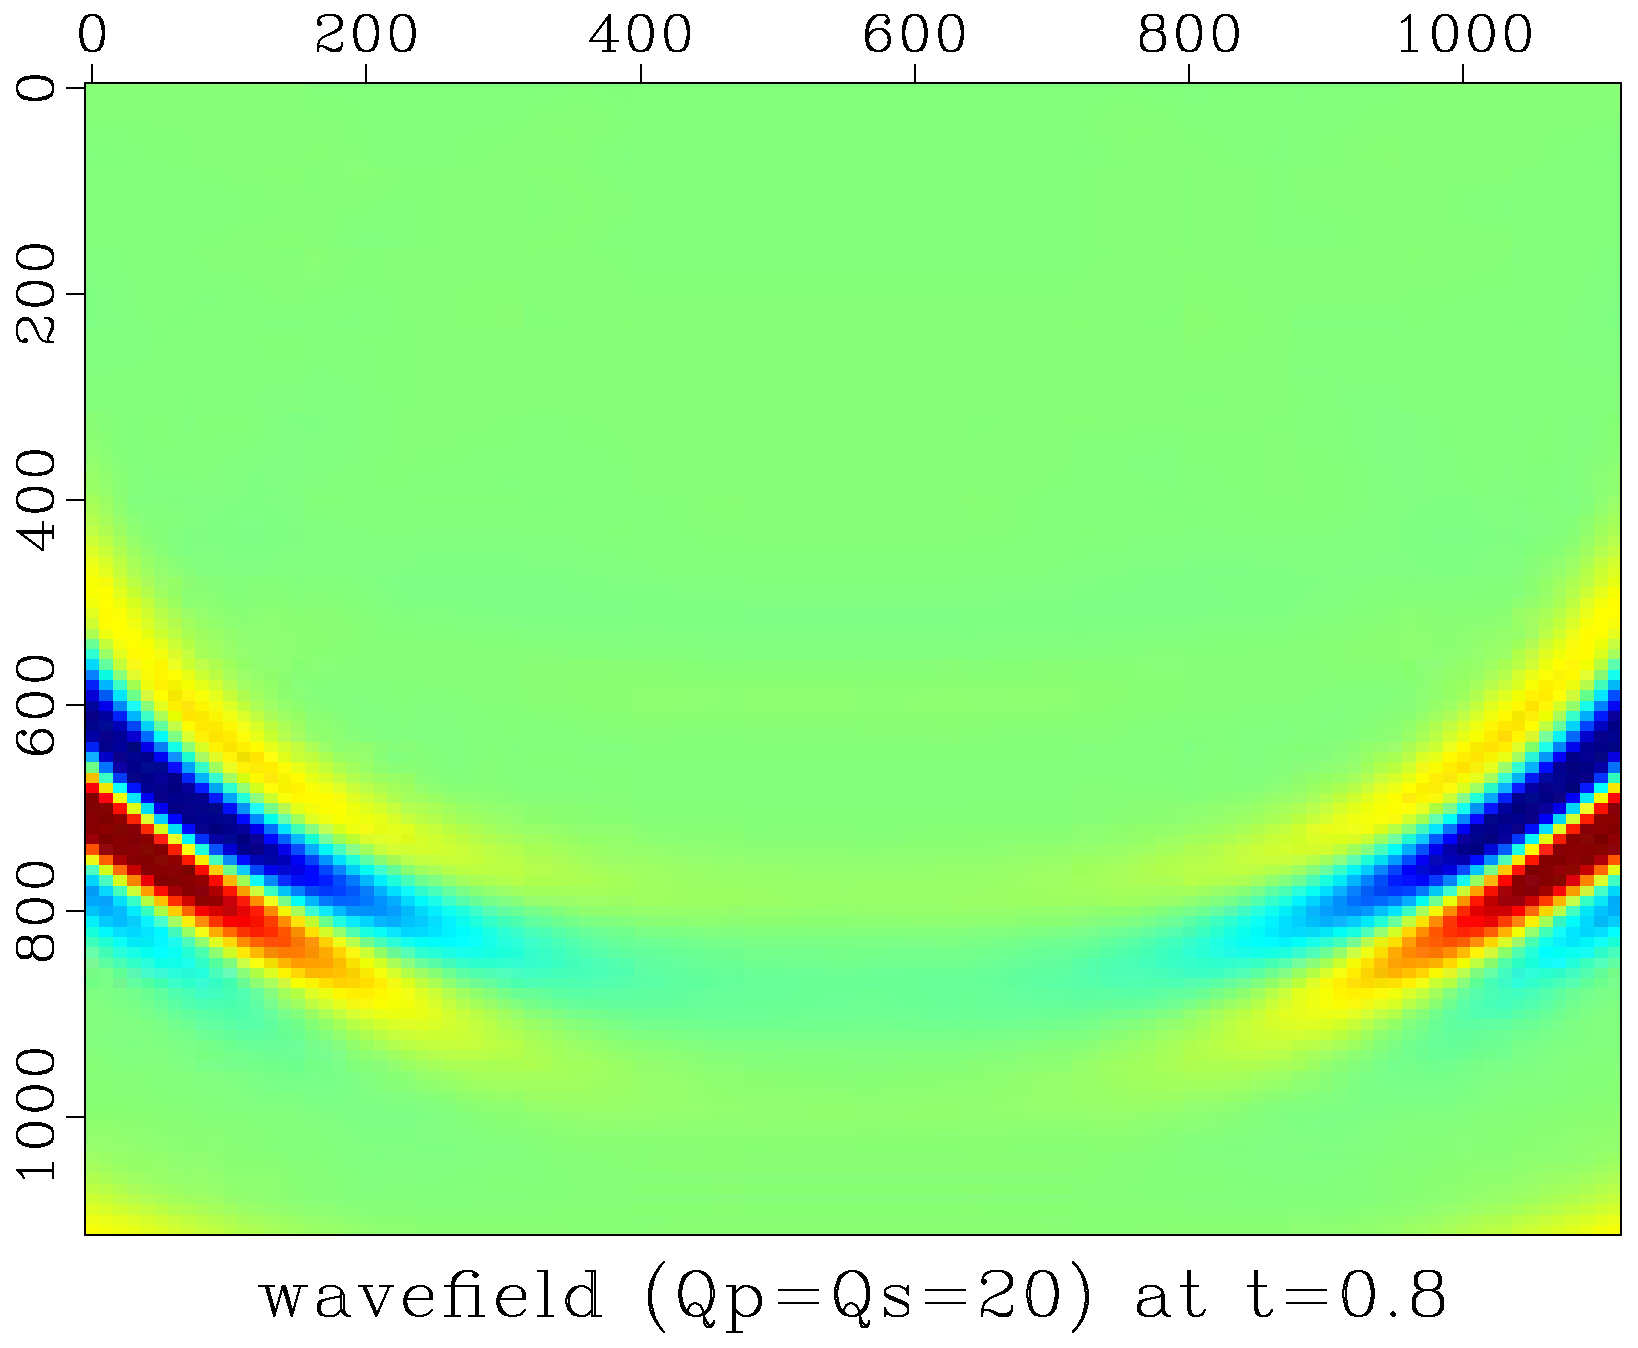
\includegraphics[height=1.3in]{./fig/q20.pdf}
        \caption{Wavefield with attenuation}
        \label{fig:with-attenuation}
    \end{subfigure}
    ~
    \begin{subfigure}[b]{0.3\textwidth}
        \centering
        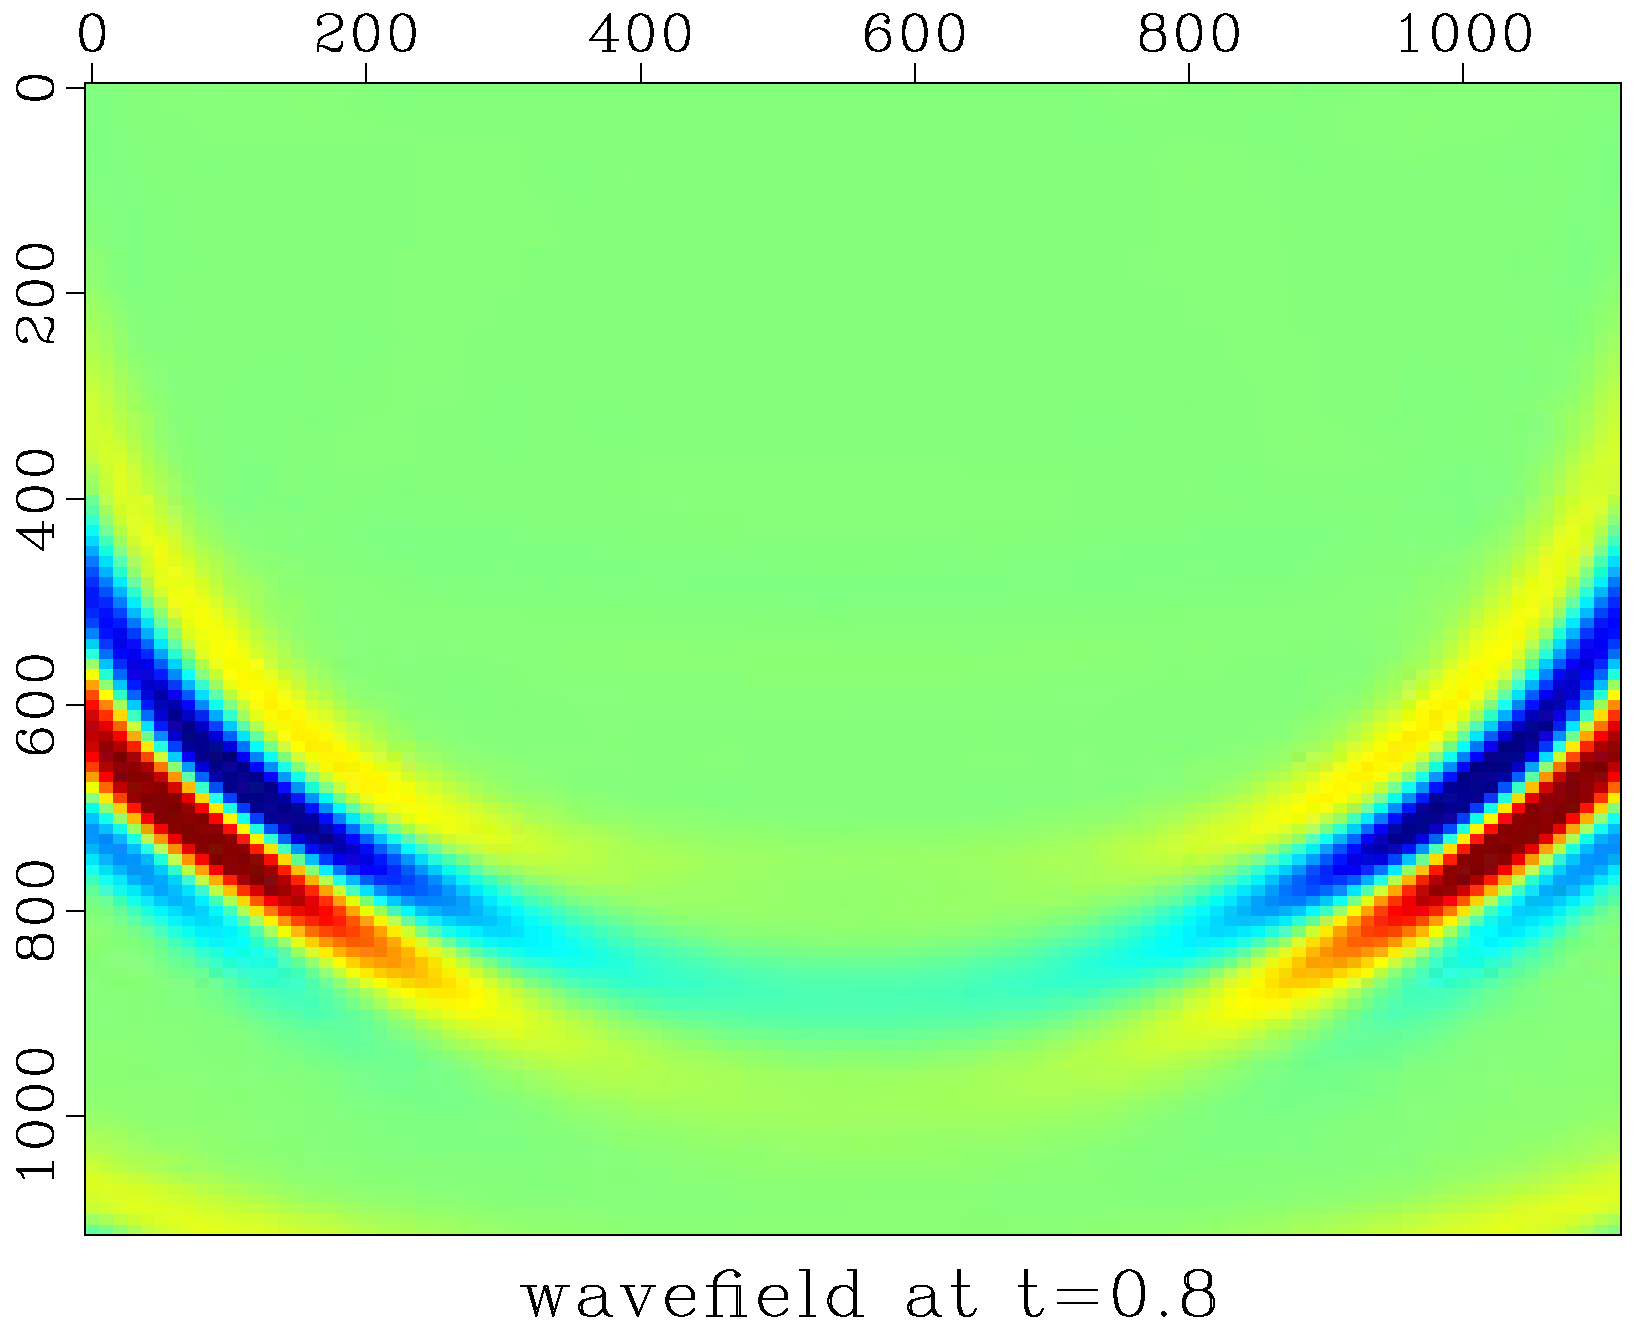
\includegraphics[height=1.3in]{./fig/std.pdf}
        \caption{Wavefield without attenuation}
        \label{fig:without-attenuation}
    \end{subfigure}%
    ~
    \begin{subfigure}[b]{0.3\textwidth}
        \centering
        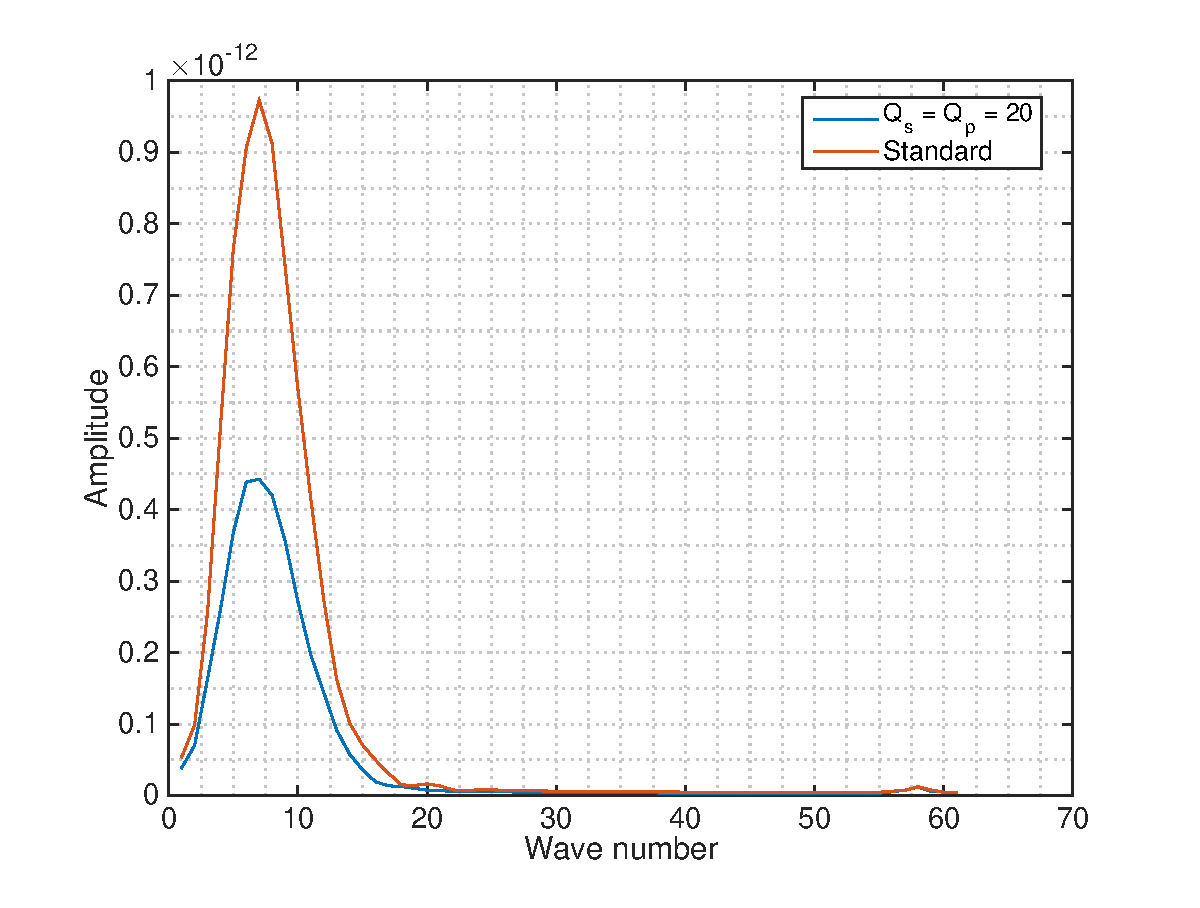
\includegraphics[height=1.3in]{./fig/spec.eps}
        \caption{Spectrum of the wavefields}
        \label{fig:spectrum}
    \end{subfigure}
    \caption{Wavefields with and without attenuation.}
\end{figure}

\subsection{Performance}

We propagate the wavefield in the 3D domain of size $700\times700\times700$ for 6000 time steps to measure the performance. Figure \ref{fig:gpu-speedup} shows the performance speedup of 1-4 K40 GPUs over one 24-core CPU node. The GPU design among 4 K40 accelerator cards can improve the performance of the computational part by up to 96 times, and improve the overall performance by up to 63 times. Note that the CPU design is also tuned by using multi-threading and vectorization. Figure \ref{fig:q-speedup} shows the speedup factor, which is  defined as the number of grid cells times time steps, as a function of propagation time for different Q values. We can see that the longer the time records, we more significant performance speedup we achieve.  Combing the two tricks as well as the GPU-based optimizations, we can achieve a performance speedup over 60 to 200 times as a function of Q.

\begin{figure}[h]
    \centering
    \begin{subfigure}[b]{0.4\textwidth}
        \centering
        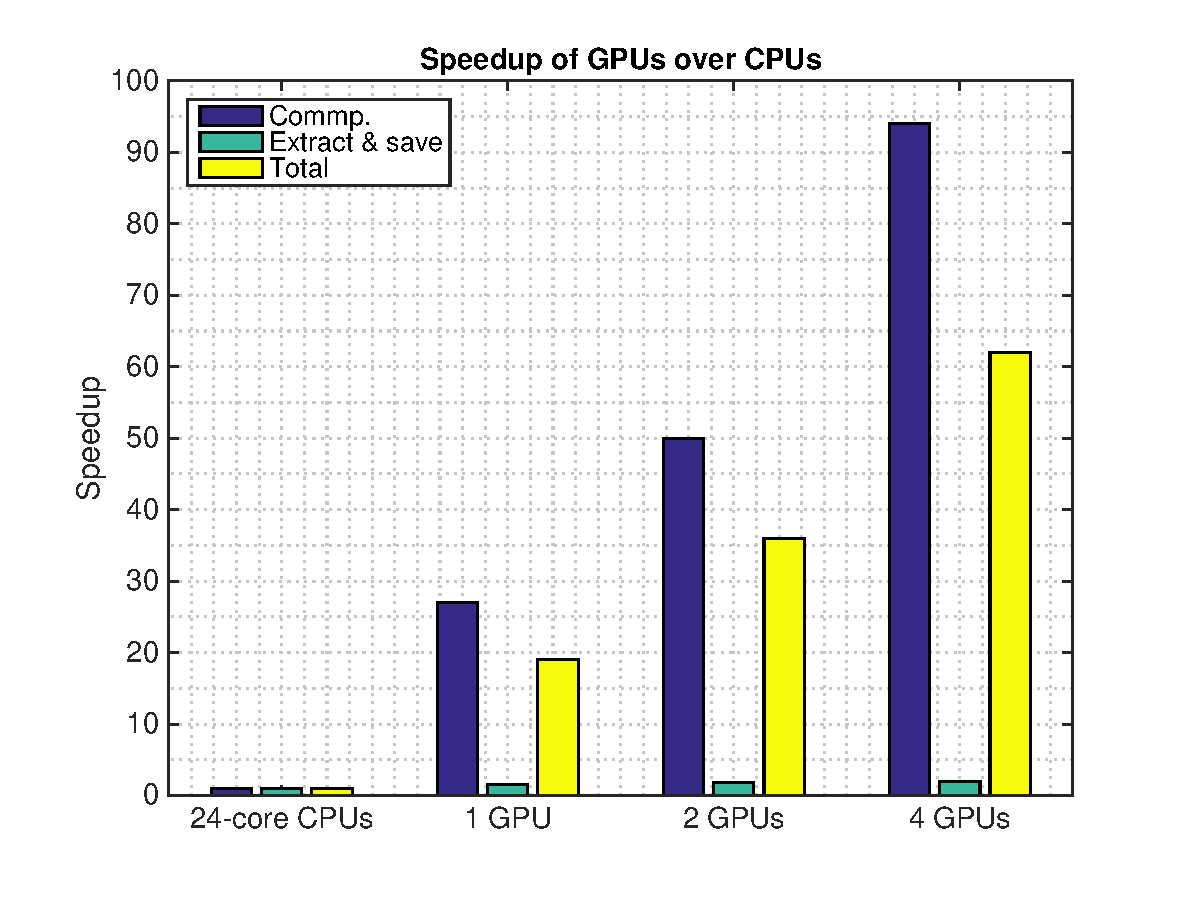
\includegraphics[height=1.5in]{./fig/speedup.eps}
        \caption{Speedup with GPU optimizations}
        \label{fig:gpu-speedup}
    \end{subfigure}%
    ~
    \begin{subfigure}[b]{0.4\textwidth}
        \centering
        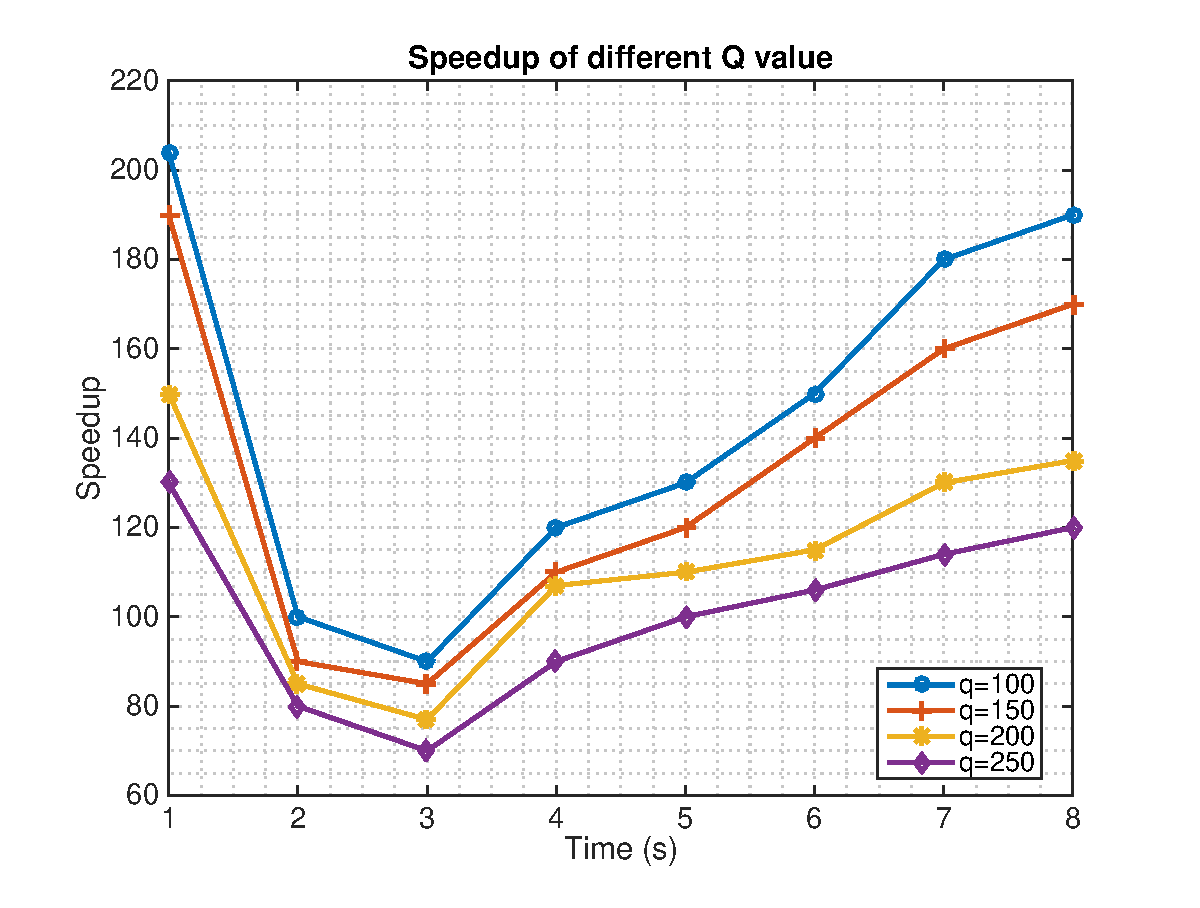
\includegraphics[height=1.5in]{./fig/speedup_q.eps}
        \caption{Speedup of different Q value}
        \label{fig:q-speedup}
    \end{subfigure}
    \caption{Performance speedup}
\end{figure}

\section{Conclusions}

This work manages to boost the performance the wave propagation in 3D elastic scenarios by approximating the Q propagation and using GPU platforms. We first extends the constant-Q formulation from the 2D viscoelastic to 3D viscoelastic case. Different optimization techniques on GPUs are then described for a high performance modeling kernel. We also propose a set of tricks to reduce the computation to further reduce computations. The experimental results show that we can achieve significant performance speedup by 60 to 200 times over the CPU-based solution.


\bibliography{bob}


\end{document}

